\documentclass[dissertation.tex]{subfiles}
\begin{document}

\chapter{Large-scale subjective evaluation}

\cite{pearce2001towards} addresses difficulty in quantitative evaluation,
suggesting the use of a learned critic in a manner similar to GANs
\cite{goodfellow2014generative}. In a later report,
\cite{pearce2002motivations} attribute difficulty in evaluation due to lack
aim: algorithmic composition, design of compositional tools, and computational
modelling of musical styles or music cognition all have different motivations
and should thus be evaluated differently.

Following advice of \cite{pearce2002motivations}, we identify our key
motivation as algorithmic composition: generation of novel compositions.
To evaluate our success, we employ a subjective evaluation method.

\cite{ariza2009} criticizes a musical Turing test as providing little data about
how to improve the system, suggesting that listener studies using music experts
may be more insightful.

\section{Evaluation framework design}

\subsection{Software architecture}

The frontend utilizes React and Redux, allowing us to collect fine-grained user
action data. Azure App Service is used to host an Express web-service which
randomizes experimental questions and collects responses. The data is stored to
Azure Data Storage and processed in batch MapReduce using Azure HDInsight.

\subsection{User interface}


The landing page for \url{http://bachbot.com/} is shown in \autoref{fig:bachbot-front-page}.

\begin{figure}[htpb]
  \centering
  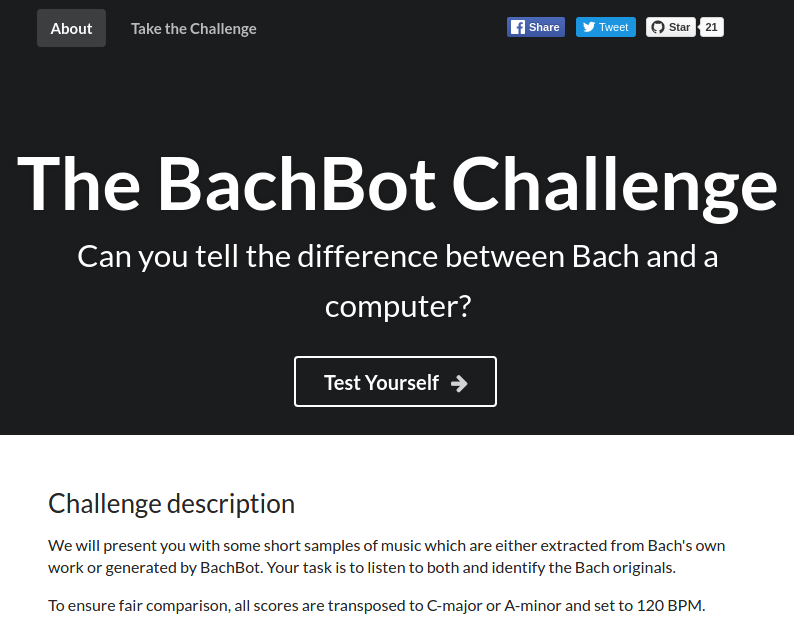
\includegraphics[width=1.0\linewidth]{Figures/bachbot-front-page.png}
  \caption{The first page seen by a visitor of \url{http://bachbot.com}}
  \label{fig:bachbot-front-page}
\end{figure}

Clicking ``Test Yourself'' redirects the participant to a user information form
(\autoref{fig:user-info-form}) where users self-report their age
group prior music experience into the categories shown.

\begin{figure}[htpb]
  \centering
  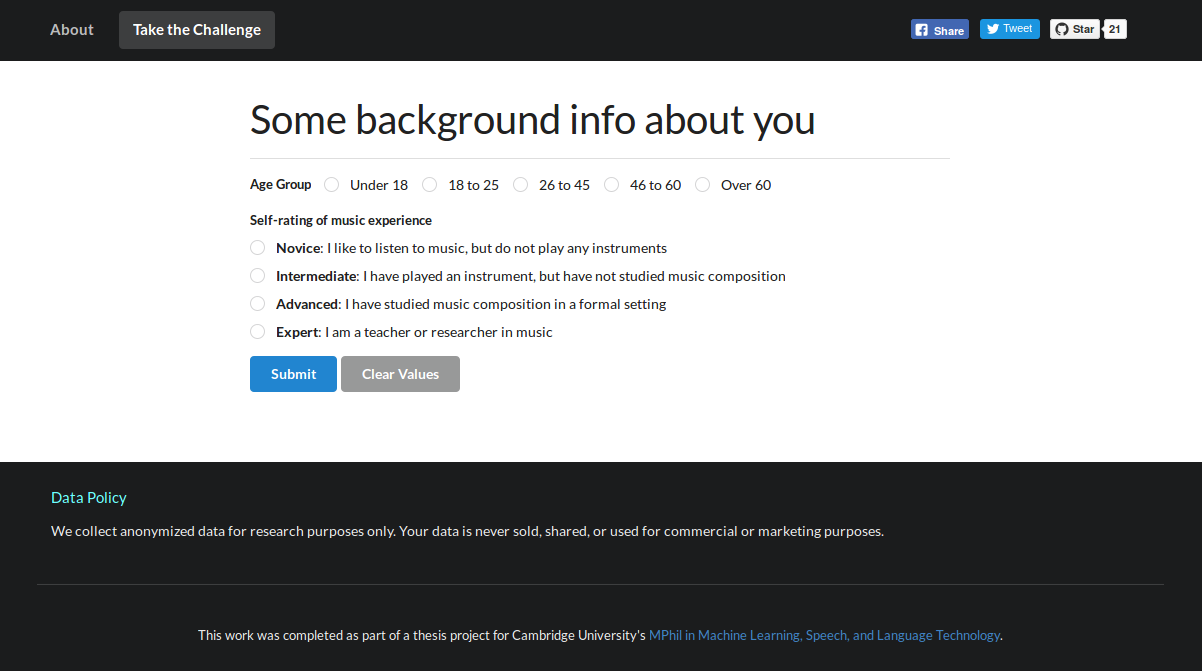
\includegraphics[width=1.0\linewidth]{Figures/user-info-form.png}
  \caption{User information form presented after clicking ``Test Yourself''}
  \label{fig:user-info-form}
\end{figure}

After submitting the background form, users were redirected to the question
response page shown in \autoref{fig:question-screen}. This page contains two
audio samples, one extracted from Bach and one generated by BachBot, and users
were asked to select the sample which sounds most similar to Bach. Users were
asked to provide five consecutive answers and then the overall percentage
correct was reported.

\begin{figure}[htpb]
  \centering
  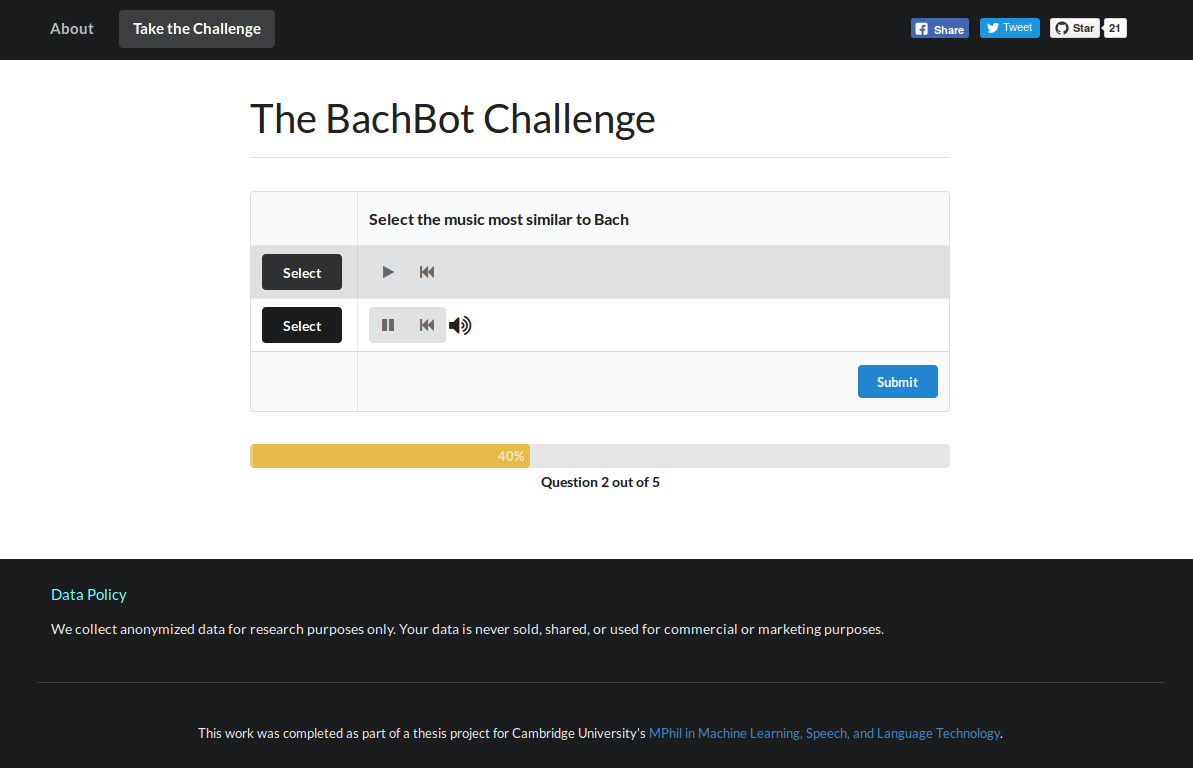
\includegraphics[width=1.0\linewidth]{Figures/question-screen.png}
  \caption{Question response interface used for all questions}
  \label{fig:question-screen}
\end{figure}

\subsection{Question generation}

Questions were generated for both harmonizations (using the same abbreviations
as defined in \todo{ref}) as well as original compositions (denoted SATB as all parts
are generated). For each question, a random chorale was selected without
replacement from the corpus and paired with a corresponding harmonization.
SATB sampls were paired with chorales randomly sampled from the corpus. The
five question answered by any given participant were comprised of one S/A/T/B
question chosen at random, one AT question, one ATB question, and two original
compositions. See
\autoref{tab:bachbot-com-question-distribtion} for details.

\begin{table}[htpb]
  \centering
  \begin{tabular}{lrr}
    \toprule
    Question Type & \# Questions &  Expected \# responses / participant \\
    \midrule
    S        & 2  & 0.25 \\
    A        & 2  & 0.25 \\
    T        & 2  & 0.25 \\
    B        & 2  & 0.25 \\
    AT       & 8  & 1 \\
    ATB      & 8  & 1 \\
    SATB     & 12 & 2 \\
    \bottomrule
  \end{tabular}
  \caption{Composition of questions on \url{http://bachbot.com}}
  \label{tab:bachbot-com-question-distribtion}
\end{table}

\section{Results}

\subsection{Participant backgrounds and demographics}

\begin{figure}[htpb]
  \centering
  \begin{subfigure}[b]{0.98\textwidth}
    \centering
    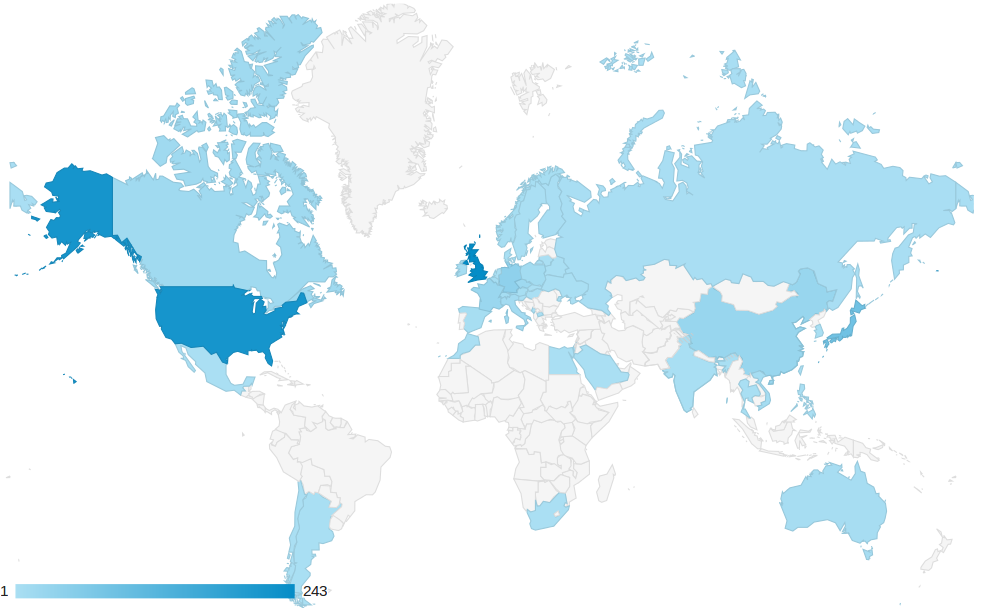
\includegraphics[width=1.0\linewidth]{Figures/participants-by-country.png}
  \end{subfigure}
  \begin{subfigure}[c]{0.55\textwidth}
    \centering
    \hspace{-1cm}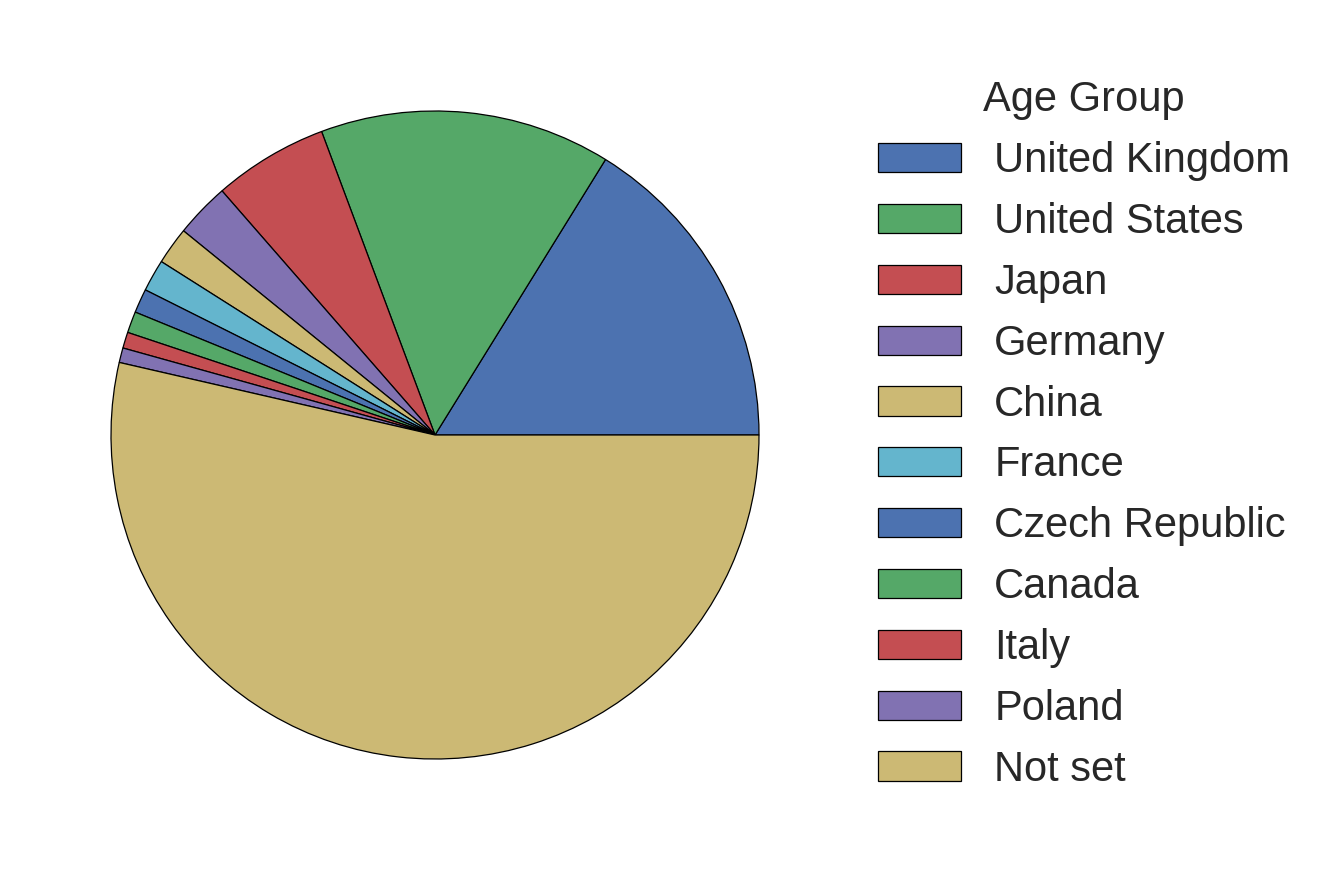
\includegraphics[width=3in]{Figures/user-demographics-pie.png}
  \end{subfigure}
  \begin{subfigure}[c]{0.44\textwidth}
    \centering
    \begin{tabular}{lrr}
\toprule
Country        &  Responses       &  Proportion \\
\midrule
UK             &       243 &            16.0\% \\
US             &       218 &            15.0\% \\
Japan          &        86 &             6.0\% \\
Germany        &        41 &             3.0\% \\
China          &        28 &             2.0\% \\
France         &        24 &             2.0\% \\
Czechia        &        18 &             1.0\% \\
Canada         &        16 &             1.0\% \\
Italy          &        12 &             1.0\% \\
Poland         &        11 &             1.0\% \\
Not set        &       805 &            54.0\% \\
\bottomrule
\end{tabular}

  \end{subfigure}
  \caption{Geographic distribution of participants}
  \label{fig:user-demographics-pie}
\end{figure}

\begin{figure}[htpb]
  \centering
  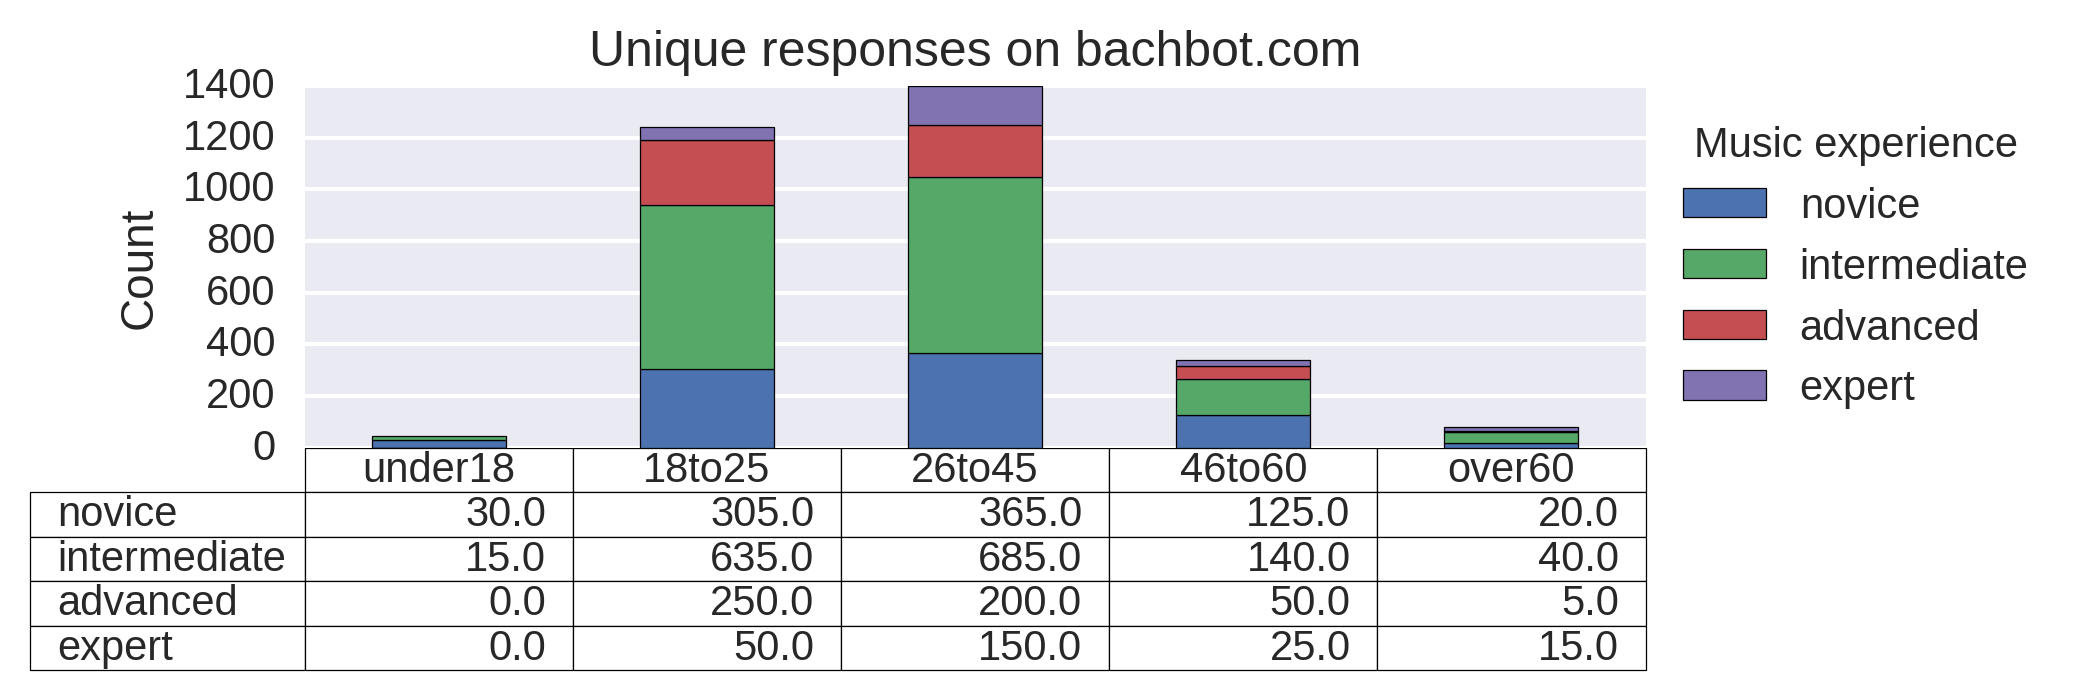
\includegraphics[width=\textwidth]{Figures/responses-ageGroup-musicExperience.png}
  \caption{Demographic breakdown of participants by age group and music experience}
  \label{fig:responses-ageGroup-musicExperience}
\end{figure}

\todo{\autoref{fig:responses-mask} suggests performance is weakest on
  harmonizations. Unsurprising because we only do 1-best and don't account
  for future. Bidirectional LSTM or N-best lattice search (reference marcin)
  would do better}
\begin{figure}[htpb]
  \centering
  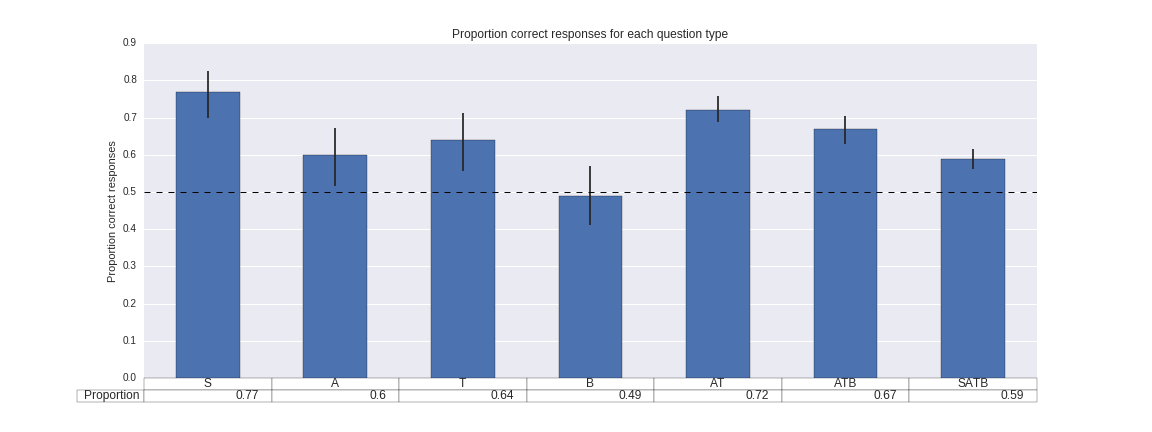
\includegraphics[width=0.8\textwidth]{Figures/responses-mask.png}
  \caption{Figures/responses-Mask}
  \label{fig:responses-mask}
\end{figure}

\begin{figure}[htpb]
  \centering
  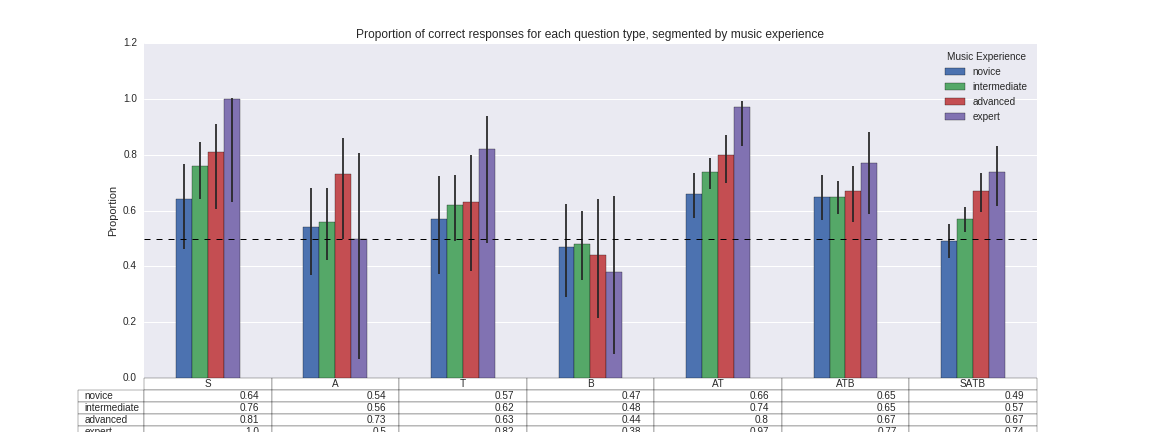
\includegraphics[width=1.0\textwidth]{Figures/responses-mask-musicExperience.png}
  \caption{Figures/responses-mask-MusicExperience}
  \label{fig:responses-mask-musicExperience}
\end{figure}

\begin{figure}[htpb]
  \centering
  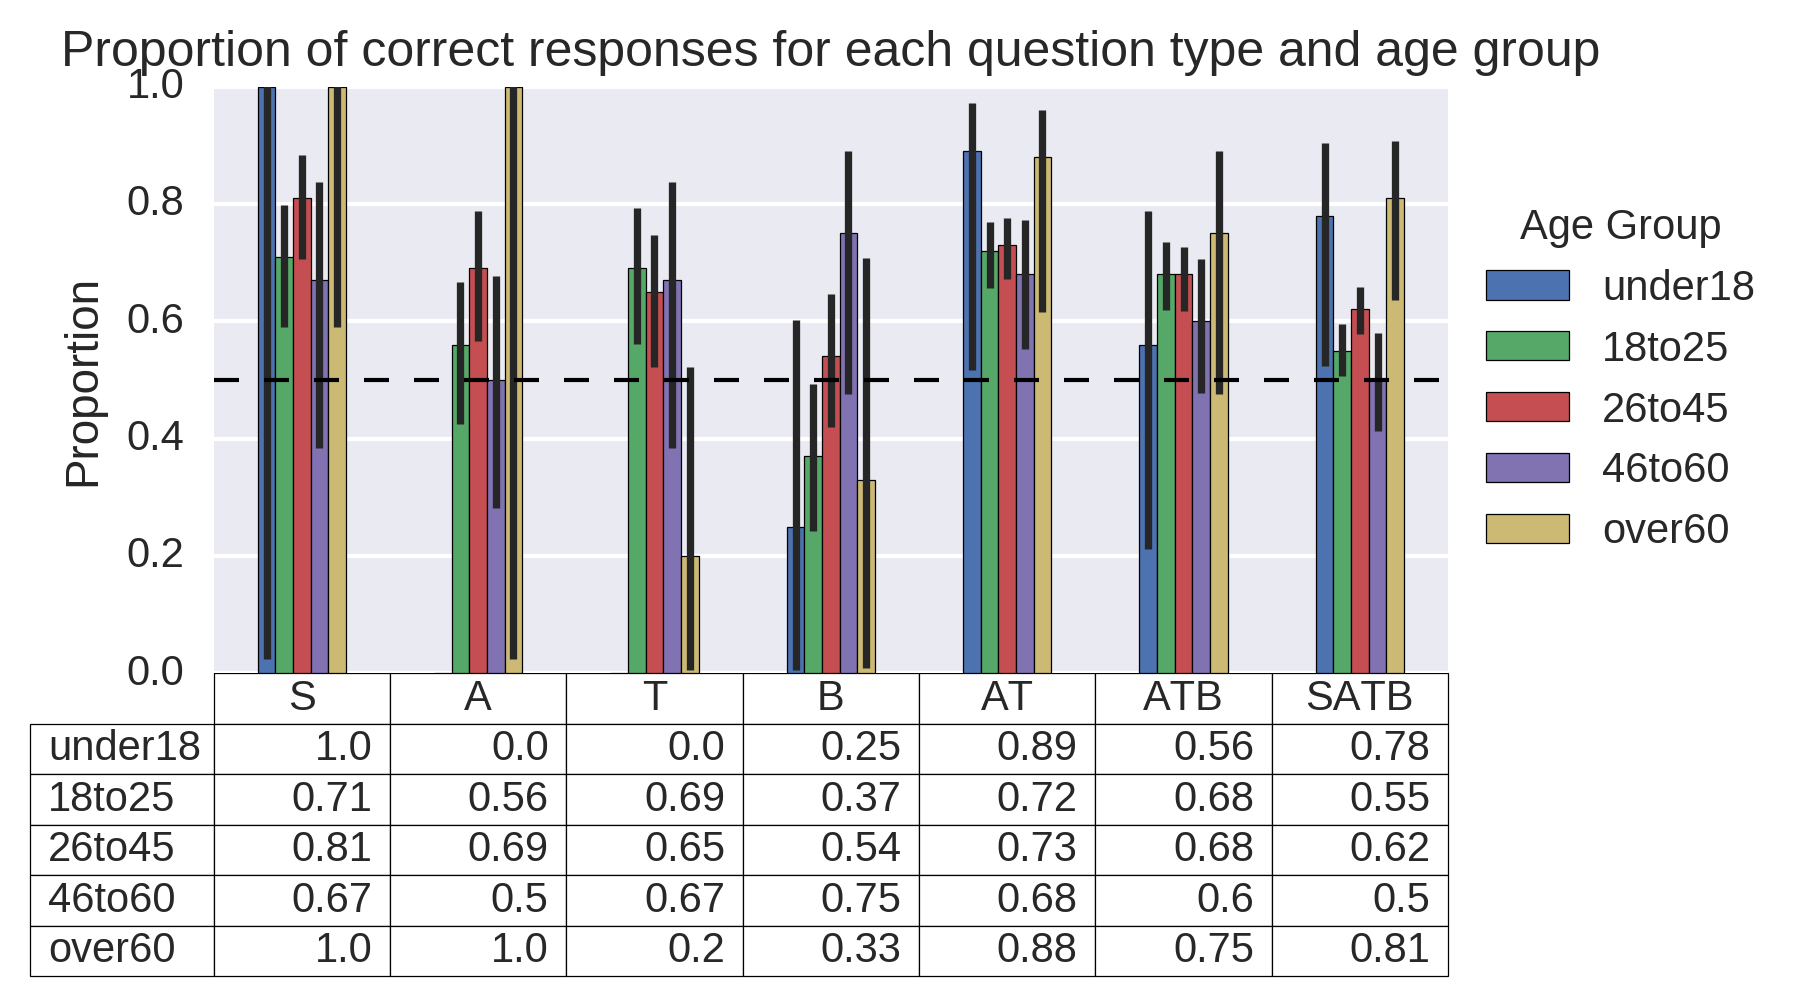
\includegraphics[width=1.0\textwidth]{Figures/responses-mask-agegroup.png}
  \caption{Figures/responses-mask-Agegroup}
  \label{fig:responses-mask-agegroup}
\end{figure}

\begin{figure}[htpb]
  \centering
  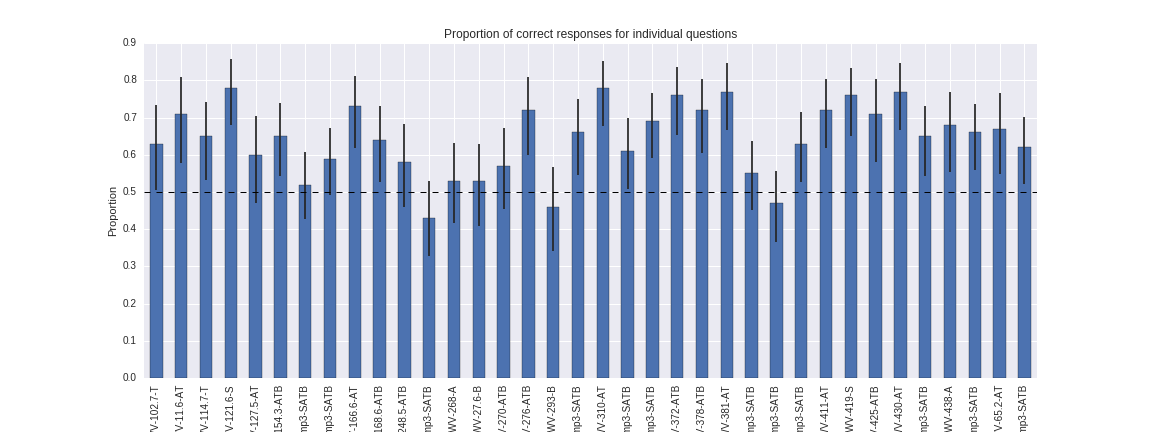
\includegraphics[width=0.8\linewidth]{Figures/responses-name.png}
  \caption{Proportion of correct responses broken down by individual questions.}
  \label{fig:responses-name}
\end{figure}

\todo{Analyze why bad questions in \autoref{fig:responses-name} are happening}

\section{User feedback}

The modulations and part writing were the giveaway for me (and once or twice the phrasing)

Got 5/5. The trick is to listen for the unnatural pauses at regular intervals.

Cool project, I scored 100\% so I'm quite pleased with myself ;o) I do
play an instrument although I'm not classical trained. If I had an
inkling to why I could choose the background phrasing of the Bach
pieces is far more elegant than the computer generated pieces.

@samim @feynmanliang really impressive! If I didn't know about counterpoint that quiz would've stumped me



\printbibliography

\end{document}
